% !TeX spellcheck = pl_PL

\rozdzial

%%%%%%%%%%%%%%%%%%%%%%%%%%%%%%%%%%%%%%%%%%%%%%%%%%%%%%%%%%%%%%%%%%%%%%%
\section{Wyszukiwanie}
\label{wyszukiwanie}

W części \textbf{"Wyszukiwanie"} znajdują się funkcje związane ze statystyką i wyszukiwaniem (rys. \ref{menuWyszukiwanie}):
\begin{itemize}
	\item \textbf{Statystyka wzorcowań} - statystyki wzorcowań, wystawionych świadectw, przyjętych przyrządów (rozdz. \ref{stat_wzor}).
	\item  \textbf{Statystyki zleceniodawców} - wszelkie wyszukiwania i statystyki związane ze zleceniodawcami: wyszukiwanie aktywnych i nieaktywnych zleceniodawców, wyszukiwanie zleceniodawców posiadających dany typ przyrządu, czy wyszukiwanie wszystkich przyrządów danego zleceniodawcy (rozdz. \ref{stat_zleceniodawcy}).
	\item \textbf{Historia wyników wzorcowań przyrządów} - porównanie wyników wzorcowania w danym zakresie dla wybranego przyrządu (moc dawki, dawka, emisja powierzchniowa) - rozdz. \ref{historia_wzorcowań}.
	\item \textbf{Przyrządy przyjęte do wzorcowania w danym okresie} - wyszukiwanie przyrządów przyjętych do wzorcowania w zadanym czasie (rozdz. \ref{przyrzady_przyjete}).
	\item \textbf{Przyrządy uszkodzone} - wyszukiwanie przyrządów uszkodzonych (rozdz. \ref{uszkodzone}).
\end{itemize}



\begin{figure}[htb]
	\centering
	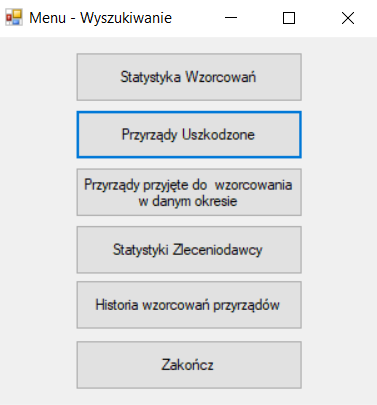
\includegraphics{obrazki/Wyszukiwanie/menu_wyszukiwanie.png}
	\caption{Menu wyszukiwanie}
	\label{menuWyszukiwanie}
\end{figure}

\subsection{Statystyka wzorcowań}
\label{stat_wzor}

Aby określić ilościowo różne rodzaje wzorcowań przyrządów w danym czasie należy w pierwszej kolejności wybrać daty odpowiadające początkowi oraz końcowi interesującego nas okresu (pola \textbf{"Szukaj od"} i \textbf{"Szukaj do"}). Po wybraniu odpowiednich dat, w tabeli poniżej, automatycznie wyświetlą się wszystkie statystyki (rys. \ref{statystykaWzorcowan}).

\textbf{TIP:} W polu \textbf{"Zleceniodawcy"} z listy rozwijanej można wybrać czy interesują nas wszyscy zleceniodawcy (\textbf{"wszyscy"}), zleceniodawcy z Instytutu Fizyki Jądrowej (\textbf{"IFJ"}), czy tylko spoza niego (\textbf{"zewnętrzni"}).

\begin{figure}[htb]
	\centering
	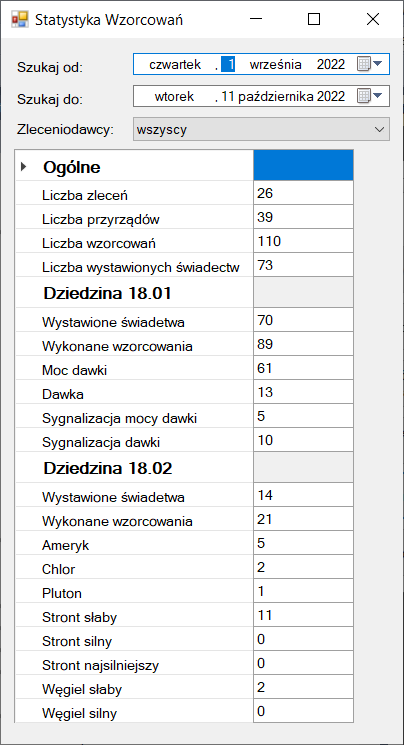
\includegraphics{obrazki/Wyszukiwanie/statystyka_wzorcowan.png}
	\caption{Okno do analizy statystyki wzorcowań przyrządów.}
	\label{statystykaWzorcowan}
\end{figure}

Poniżej zamieszczono spis wyjaśniający znaczenie poszczególnych pól.

\textbf{Ogólne:}
\begin{itemize} 
	\item \textbf{Liczba zleceń} - liczba zleceń, które zostały przyjęte w danym okresie.
	\item \textbf{Liczba przyrządów} - liczba przyrządów, które zostały przyjęte do wzorcowania w danym okresie (niekoniecznie zostały wywzorcowane).
	\item \textbf{Liczba wzorcowań} - całkowita liczba wykonanych wzorcowań w zadanym okresie (suma wszystkich wzorcowań z dziedzin 18.01 i 18.02).
	\item \textbf{Liczba wystawionych świadectw} - całkowita liczba wystawionych świadectw w zadanym okresie. Liczba ta nie pokrywa się z liczbą przyjętych przyrządów, gdyż z jednej strony nie wszystkie przyjęte w danym czasie do wzorcowania przyrządy zostały wywzorcowane (bądź nie wystawiono dla nich świadectwa - np. były zepsute). a z drugiej strony w zadanym okresie mogły zostać wystawione świadectwa przyrządów przyjętych do wzorcowania wcześniej. Całkowita liczba świadectw nie jest też bezpośrednią sumą świadectw wystawionych w dziedzinach 18.01 i 18.02, ponieważ część świadectw może zawierać wyniki wzorcowań z obu tych dziedzin jednocześnie.
\end{itemize}

\textbf{Dziedzina 18.01}
\begin{itemize}
	\item \textbf{Wystawione świadectwa} - liczba świadectw wystawionych w zadanym okresie, które przedstawiają wyniki z dziedziny 18.01. Liczba świadectw nie pokrywa się z liczbą wzorcowań, ponieważ niektóre przyrządy mogą być wykalibrowane na kilka sposobów w ramach tej samej dziedziny (np. w zakresie mocy dawki i dawki), bądź też jedno świadectwo może przedstawiać wyniki w tym samym zakresie, ale dla różnych sond.
	\item \textbf{Wykonane wzorcowania} - liczba wzorcowań wykonanych w danym okresie w dziedzinie 18.01. Jest to suma wzorcowań w zakresie mocy dawki, dawki, sygnalizacji mocy dawki i sygnalizacji dawki.
	\item \textbf{Moc dawki} - liczba wykonanych w danym okresie wzorcowań w zakresie mocy dawki.
	\item \textbf{Dawka} - liczba wykonanych w danym okresie wzorcowań w zakresie dawki.
	\item \textbf{Sygnalizacja mocy dawki} - liczba wykonanych w danym okresie wzorcowań w zakresie sygnalizacji mocy dawki.
	\item \textbf{Sygnalizacja dawki} - liczba wykonanych w danym okresie wzorcowań w zakresie sygnalizacji dawki.
\end{itemize}

\textbf{Dziedzina 18.02}
\begin{itemize}
	\item \textbf{Wystawione świadectwa} - liczba świadectw wystawionych w zadanym okresie, które przedstawiają wyniki z dziedziny 18.02. Liczba świadectw nie pokrywa się z liczbą wzorcowań, ponieważ niektóre przyrządy mogą być wykalibrowane kilkoma różnymi źródłami, bądź też jedno świadectwo może przedstawiać wyniki dla różnych sond.
	\item \textbf{Wykonane wzorcowania} - liczba wzorcowań wykonanych w danym okresie w dziedzinie 18.02. Jest to suma wzorcowań w zakresie emisji powierzchniowej wykonanych za pomocą poszczególnych źródeł.
	\item \textbf{Ameryk} - liczba wykonanych w danym okresie wzorcowań w zakresie emisji powierzchniowej źródłem Am-241.
	\item \textbf{Chlor} - liczba wykonanych w danym okresie wzorcowań w zakresie emisji powierzchniowej źródłem Cl-36.
	\item \textbf{Pluton} - liczba wykonanych w danym okresie wzorcowań w zakresie emisji powierzchniowej źródłem Pu-239.
	\item \textbf{Stront słaby} - liczba wykonanych w danym okresie wzorcowań w zakresie emisji powierzchniowej najsłabszym źródłem Sr-90/Y-90.
	\item \textbf{Stront silny} - liczba wykonanych w danym okresie wzorcowań w zakresie emisji powierzchniowej silnym źródłem Sr-90/Y-90.
	\item \textbf{Stront słaby} - liczba wykonanych w danym okresie wzorcowań w zakresie emisji powierzchniowej najsilniejszym źródłem Sr-90/Y-90.
	\item \textbf{Węgiel słaby} - liczba wykonanych w danym okresie wzorcowań w zakresie emisji powierzchniowej słabszym źródłem C-14.
	\item \textbf{Węgiel silny} - liczba wykonanych w danym okresie wzorcowań w zakresie emisji powierzchniowej silniejszym źródłem C-14.
\end{itemize}

\subsection{Statystyki zleceniodawców}
\label{stat_zleceniodawcy}

W menu \textbf{"Statystyki zleceniodawców"} (rys. \ref{menuStatystykiZleceniodawcy}) można znaleźć następujące funkcje:
\begin{itemize}
	\item \textbf{Liczba przyrządów zleceniodawców w danym okresie} - wypisanie wszystkich zleceniodawców, którzy przysłali przyrządy do wzorcowania w danym okresie, wraz z liczbą przyrządów.
	\item \textbf{Nieaktywni zleceniodawcy} - wyszukiwanie zleceniodawców, którzy zaprzestali przysyłania przyrządów do wzorcowania.
	\item \textbf{Zleceniodawcy posiadający dany typ przyrządu} - wyszukiwanie zleceniodawców, którzy posiadają dany typ przyrządu
	\item \textbf{Przyrządy danego zleceniodawcy} - wyszukiwanie wszystkich przyrządów danego zleceniodawcy.
\end{itemize}

\begin{figure}[htb]
	\centering
	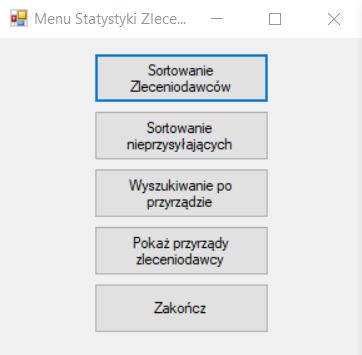
\includegraphics{obrazki/Wyszukiwanie/Zleceniodawcy/menu_statystyki_zleceniodawcow.png}
	\caption{Menu statystyk związanych ze zleceniodawcami.}
	\label{menuStatystykiZleceniodawcy}
\end{figure}

\subsubsection{Liczba przyrządów zleceniodawców w danym okresie}
\label{sort_zleceniodawcow}

Ten moduł umożliwia wyszukanie zleceniodawców, którzy w wybranym okresie przysłali swoje przyrządy do wzorcowania. W polach oznaczonych \textbf{"Między datami:"} należy podać interesujący nas zakres dat (rys. \ref{aktywniZleceniodawcy}). Poniżej w tabeli pojawią się ID oraz nazwy zleceniodawców, których przyrządy zostały przyjęte do laboratorium wzorcowania. Dodatkowo w kolumnie \textbf{"Liczba przyrządów"} podana będzie liczba przyjętych przyrządów każdego ze zleceniodawców.

\textbf{TIP:} Dane w tabeli można dowolnie posortować klikając w nagłówek wybranej kolumny.

\begin{figure}[htb]
	\centering
	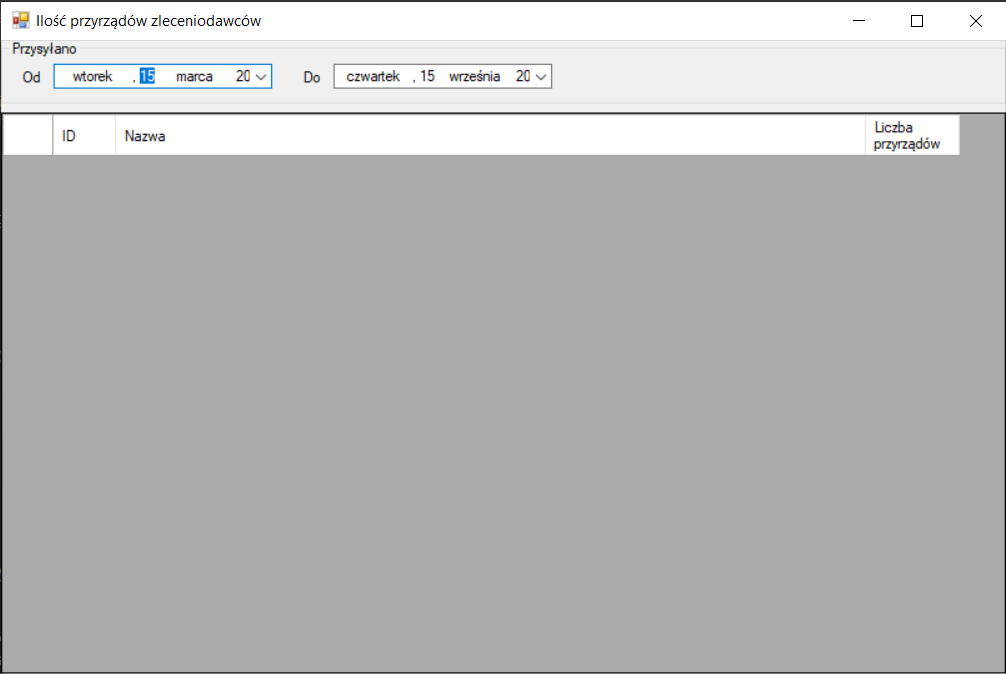
\includegraphics[width=\columnwidth]{obrazki/Wyszukiwanie/Zleceniodawcy/ilosc_przyrzadow_zleceniodawcow.png}
	\caption{Okno wyszukiwania zleceniodawców aktywnych w zadanym okresie.}
	\label{aktywniZleceniodawcy}
\end{figure}

\subsubsection{Nieaktywni zleceniodawcy}
\label{sort_nieprzysylajacych}

Ta część programu pozwala na wyszukanie nieaktywnych już zleceniodawców, tj. zleceniodawców, którzy zaprzestali przysyłać swoje przyrządy do wzorcowania.

W części "Przysłano" w polach \textbf{"Między datami"} należy wybrać zakres dat, kiedy zleceniodawca przysłał swoje przyrządy do wzorcowania co najmniej raz. W części "Nie przysłano" należy w polach \textbf{"Między datami"} podać daty, w zakresie których dany zleceniodawca był nieaktywny (nie przysłał żadnego przyrządu do wzorcowania). Następnie należy wcisnąć przycisk \textbf{"Szukaj"}. W tabeli pojawią się dane (ID i nazwa) wszystkich zleceniodawców spełniających powyższe kryteria (rys. \ref{nieaktywniZleceniodawcy}).

\textbf{TIP:} Funkcję tę można wykorzystać zarówno do wyszukania zleceniodawców, którzy zaprzestali współpracy z laboratorium, jak i do wyszukania tych, którzy są nowymi klientami. W tym drugim przypadku należy w części \textbf{"Przysłano"} wybrać daty późniejsze niż w części \textbf{"Nie przysłano"}.

\begin{figure}[htb]
	\centering
	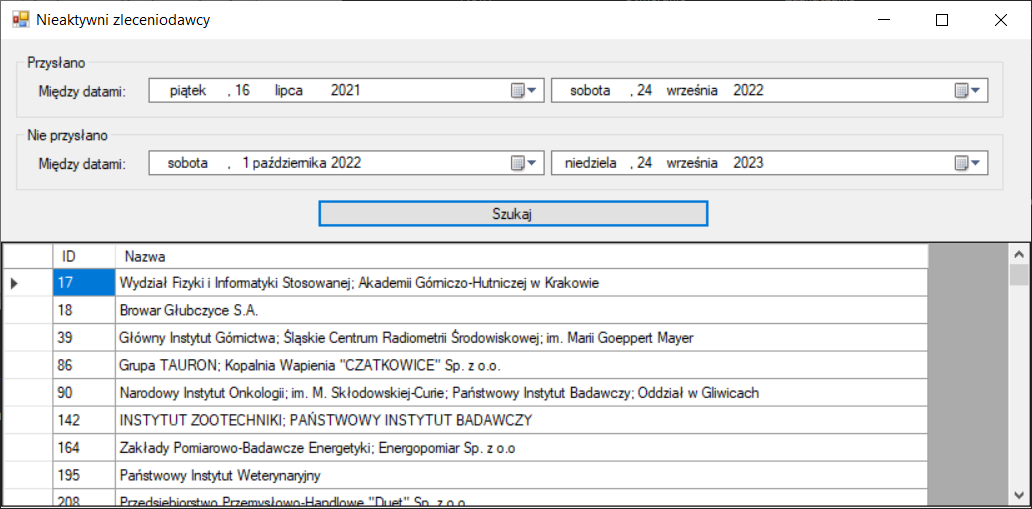
\includegraphics[width=\columnwidth]{obrazki/Wyszukiwanie/Zleceniodawcy/nieaktywni_zleceniodawcy.png}
	\caption{Okno wyszukiwania nieaktywnych zleceniodawców.}
	\label{nieaktywniZleceniodawcy}
\end{figure}

\subsubsection{Zleceniodawcy posiadający dany typ przyrządu}
\label{wysz_po_przyrzadzie}

W tym oknie (rys. \ref{wyszPoPrzyrzadzie}) można wyszukać wszystkich zleceniodawców posiadających dany typ przyrządu. W tym celu w polu \textbf{"Typ przyrządu"} należy wpisać interesujący nas typ przyrządu. W tabeli pojawią się ID i nazwy zleceniodawców, którzy wzorcowali w laboratorium przyrząd szukanego przez nas typu. 

\textbf{TIP}: Po wpisaniu kilku liter nazwy szukanego typu, można wyszukać go na liście rozwijanej. Wielkość liter nie ma znaczenia.

\begin{figure}[htb]
	\centering
	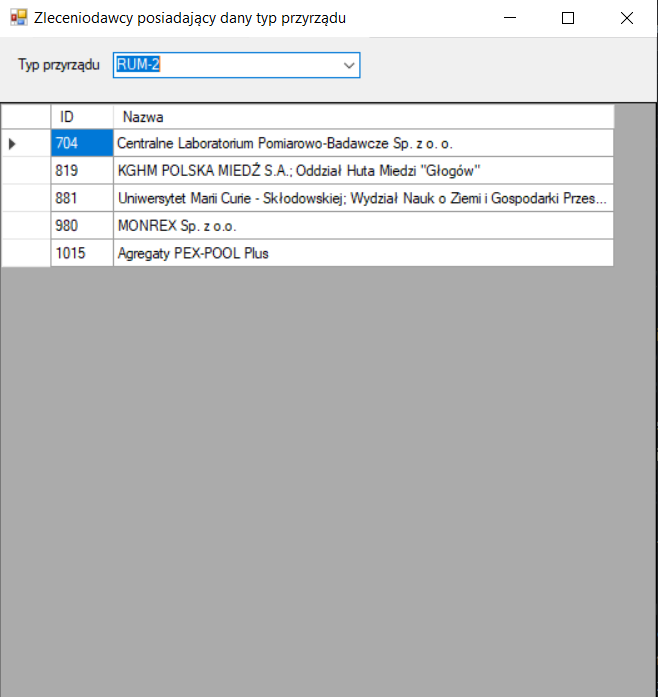
\includegraphics{obrazki/Wyszukiwanie/Zleceniodawcy/wyszukiwanie_po_przyrzadzie.png}
	\caption{Okno wyszukiwania zleceniodawców posiadających dany typ przyrządu.}
	\label{wyszPoPrzyrzadzie}
\end{figure}

\subsubsection{Przyrządy danego zleceniodawcy}
\label{przyrz_zleceniodawcy}

W tym oknie możliwe jest wyszukanie wszystkich przyrządów danego zleceniodawcy, które były kiedykolwiek wzorcowane w naszym laboratorium (rys. \ref{przyrzadyZleceniodawcy}). Jeżeli znane jest ID zleceniodawcy (można je znaleźć np. w części Biuro - Zlecenie \ref{}) można wpisać je bezpośrednio w polu \textbf{ID}. Drugą opcją jest wpisanie nazwy zleceniodawcy w polu \textbf{"Nazwa"}. W tabeli pojawią się nazwy i numery fabryczne posiadanych przez zleceniodawcę przyrządów.

\textbf{TIP}: Po wpisaniu kilku liter nazwy, można wyszukać ją na liście rozwijanej. Wielkość liter nie ma znaczenia.

\begin{figure}[htb]
	\centering
	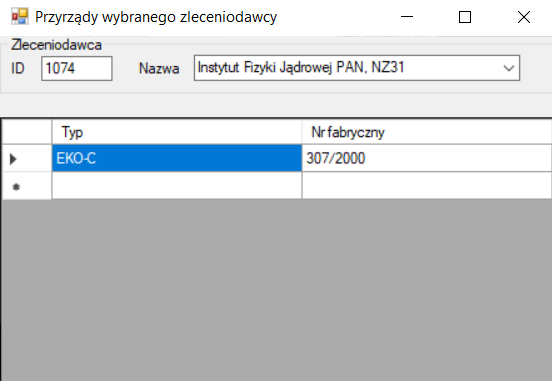
\includegraphics{obrazki/Wyszukiwanie/Zleceniodawcy/przyrzady_zleceniodawcy.png}
	\caption{Okno wyszukiwania wszystkich przyrządów wybranego zleceniodawcy.}
	\label{przyrzadyZleceniodawcy}
\end{figure}
\subsection{Historia wzorcowań przyrządów}
\label{historia_wzorcowań}

W tym oknie mamy możliwość prześledzić historię wyników wzorcowania danego przyrządu w zakresie mocy dawki, dawki oraz emisji powierzchniowej.

\begin{figure}[H]
	\centering
	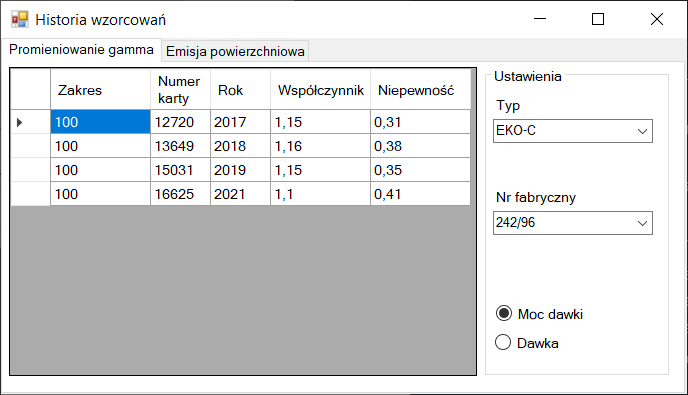
\includegraphics{obrazki/Wyszukiwanie/historia_wzorcowan_moc.png}
	\caption{Okno umożliwiające sprawdzenie historii wzorcowania danego przyrządu w zakresie dawki i mocy dawki.}
	\label{historiaWzorcowanMoc}
\end{figure}

W zakładce \textbf{"Promieniowanie gamma"} (rys. \ref{historiaWzorcowanMoc}) należy w pierwszej kolejności zaznaczyć czy chcemy otrzymać wyniki wzorcowania przyrządu w zakresie dawki czy mocy dawki. Następnie z listy rozwijanej należy wybrać typ przyrządu, a w kolejnym kroku jego numer fabryczny. W tabeli wyświetlą się znalezione dla wybranego przyrządu wyniki wzorcowania (numer karty przyjęcia, rok wzorcowania, zakres, współczynnik kalibracyjny wraz z niepewnością).

\textbf{TIP:} Po wybraniu danego typu przyrządu lista rozwijana zawierająca numery fabryczne zostaje ograniczona do numerów fabrycznych przyrządów wybranego typu.

\textbf{TIP:} Wyniki przedstawione w tabeli są domyślnie posortowane po numerze karty. Można je jednak posortować względem dowolnej kolumny klikając na nagłówek wybranej kolumny. W przypadku przyrządów posiadających więcej niż jeden zakres warto posortować wyniki właśnie po zakresie, co umożliwia łatwe porównywanie wyników wzorcowania dla poszczególnych zakresów przyrządu.

\begin{figure}[htb]
	\centering
	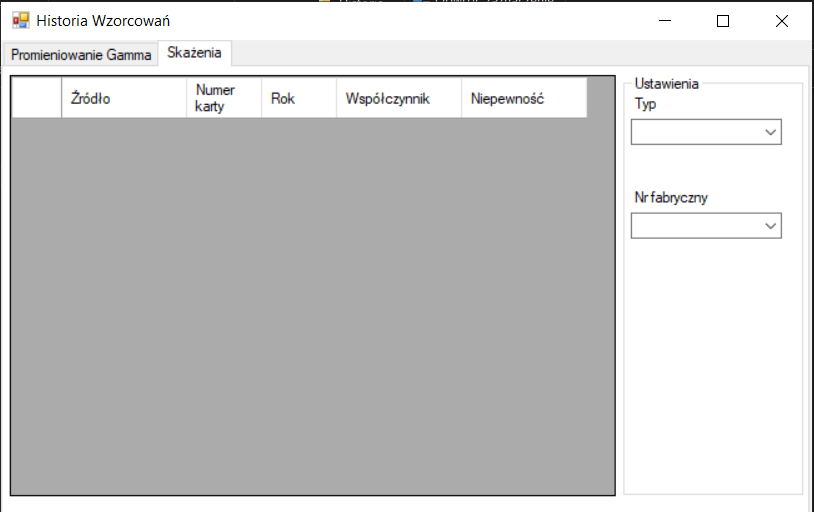
\includegraphics{obrazki/Wyszukiwanie/historia_wzorcowan_skazenia.png}
	\caption{Okno umożliwiające sprawdzenie historii wzorcowania danego przyrządu w zakresie emisji powierzchniowej.}
	\label{historiaWzorcowanSkazenia}
\end{figure}

Przeglądanie wyników wzorcowania danego przyrządu w zakresie emisji powierzchniowej odbywa się w zakładce \textbf{"Emisja powierzchniowa"}. Podobnie jak w przypadku wzorcowania promieniowaniem gamma należy w pierwszej kolejności wybrać z listy rozwijanej typ przyrządu, a następnie z kolejnej listy rozwijanej jego numer fabryczny. Dla wybranego przyrządu w tabeli wyświetlą się znalezione wyniki wzorcowania (numer karty przyjęcia, rok wzorcowania, źródło, współczynnik kalibracyjny wraz z niepewnością).

\subsection{Przyrządy przyjęte do wzorcowania w danym okresie}
\label{przyrzady_przyjete}

Aby wyświetlić informacje dotyczące typów przyrządów, które zostały przyjęte do wzorcowania w danym czasie, należy w pierwszej kolejności wybrać daty odpowiadające początkowi oraz końcowi interesującego nas okresu (pola \textbf{"Szukaj od"} i \textbf{"Szukaj do"}). Po wybraniu odpowiednich dat w tabeli poniżej automatycznie wyświetli się lista wszystkich typów przyrządów przyjętych do wzorcowania w zadanym zakresie dat wraz z ich liczbą  (rys. \ref{przyrzadyPrzyjete}).

\textbf{TIP:} Dane w tabeli można dowolnie posortować klikając w nagłówek wybranej kolumny.

\begin{figure}[htb]
	\centering
	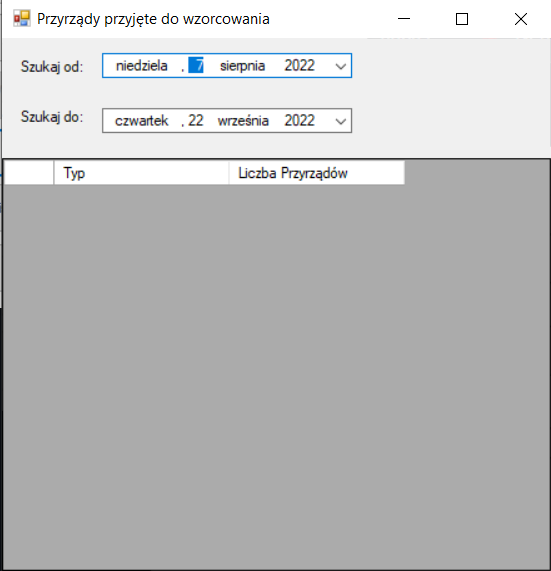
\includegraphics{obrazki/Wyszukiwanie/przyrzady_przyjete.png}
	\caption{Okno wyszukiwania przyrządów przyjętych do wzorcowania w danym okresie.}
	\label{przyrzadyPrzyjete}
\end{figure}

\subsection{Przyrządy uszkodzone}
\label{uszkodzone}

Aby wyświetlić informacje dotyczące przyrządów, których uszkodzenie zostało stwierdzone w danym czasie, należy w pierwszej kolejności wybrać daty odpowiadające początkowi oraz końcowi interesującego nas okresu (pola \textbf{"Szukaj od"} i \textbf{"Szukaj do"}). Po wybraniu odpowiednich dat w tabeli poniżej automatycznie wyświetlą się podstawowe informacje o uszkodzonych przyrządach (rys. \ref{przyrzadyUszkodzone}).  Pole w prawym górnym rogu pokazuje ogólną liczbę uszkodzonych przyrządów.

\begin{figure}[htb]
	\centering
	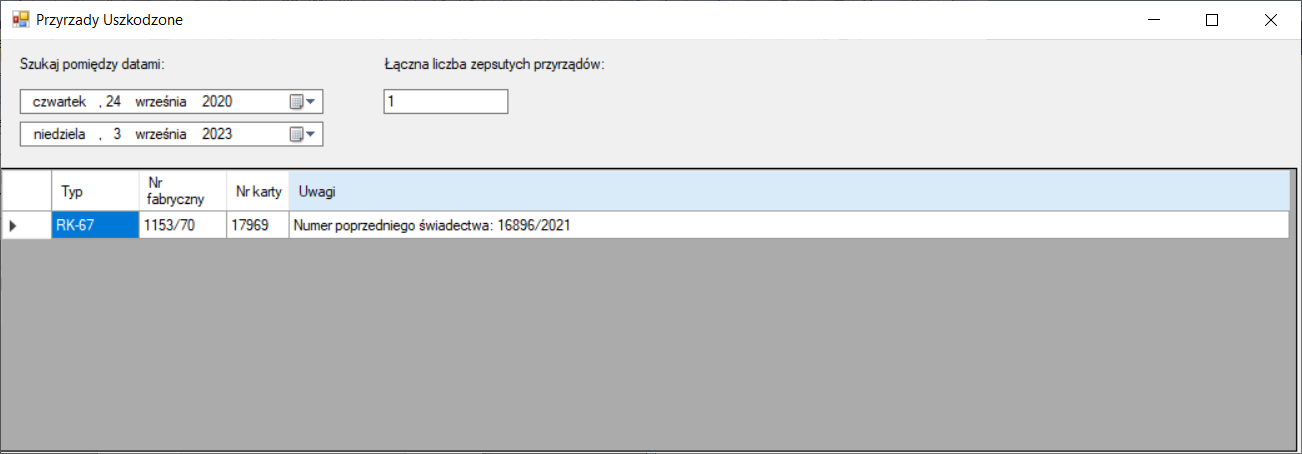
\includegraphics[width=\columnwidth]{obrazki/Wyszukiwanie/przyrzady_uszkodzone.png}
	\caption{Okno wyszukiwania przyrządów uszkodzonych w danym okresie.}
	\label{przyrzadyUszkodzone}
\end{figure}